\chapter{Dresden OCL Metrics}
\label{chapter:metrics}

\begin{flushright}
\textit{Chapter written by Claas Wilke}
\end{flushright}

This chapter describes how the Dresden OCL Metrics tool provided with Dresden
OCL can be used. A general introduction into Dresden OCL can be found in
Chapter~\ref{chapter:introduction}.
This chapter uses the \keyword{Simple Example} which is provided with 
Dresden OCL and has been introduced in Section~\ref{intro:simpleExample}. 



\section{Using Dresden OCL Metrics}

The Dresden OCL Metrics tool is a simple tool that allows to compute some
statistics for a selected or a set of selected OCL constraints.

In summary, the following metrics can be computed:

\begin{itemize}
  \item The number of constraints selected,
  \item The number of constraints by kind (Body, Definition, Derived,
  Init, Invariant, Postcondition, Precondition),
  \item The number of expressions used within the selected constraints
  (including minimum, maximum, average, and median number of expressions per
  constraint),
  \item The depth of the expressions within the selected constraints (minimum,
  maximum, average, and median),
  \item The number of if-expressions used within the selected constraints,
  \item The number of let-expressions used within the selected constraints,
  \item The number and kinds of literals used within the selected constraints,
  \item The number and kinds of iterators used within the selected constraints,
  \item The number and names of operations called within the selected
  constraints,
  \item The number and names of properties called within the selected
  constraints.
\end{itemize}

Dresden OCL Metrics consists of a single view that should be visible at the
center bottom of the Dresden OCL perspective (cf.
Fig.~\ref{pic:metrics:metrics01}). If not, the view can be opened by the menu
option \emph{Dresden OCL -> Open OCL Metrics}.

\begin{figure}[!t]
	\centering
	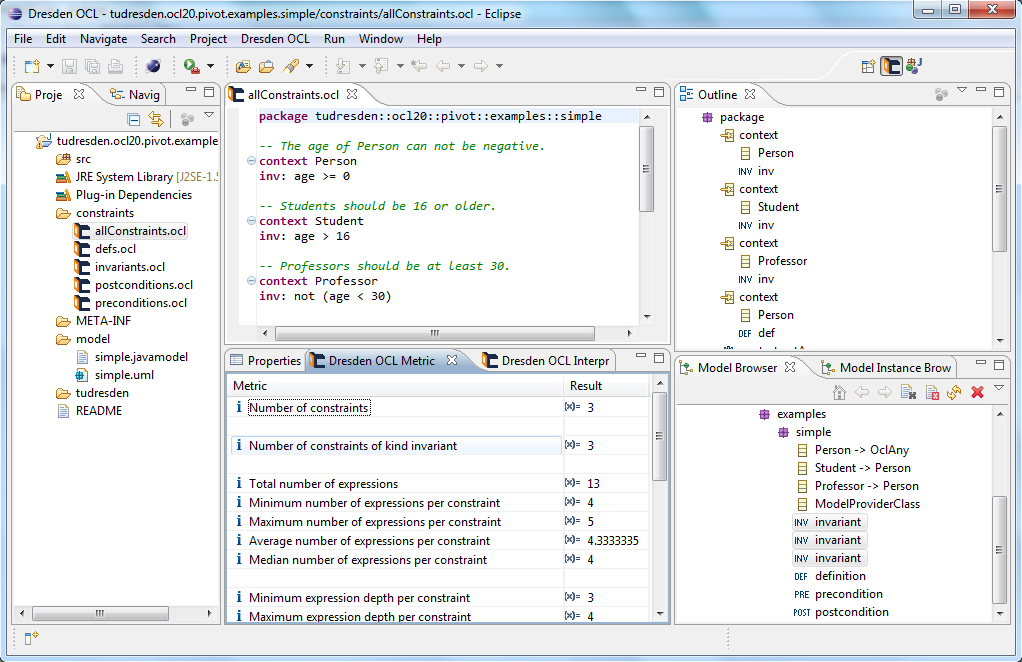
\includegraphics[width=1.0\textwidth]{figures/metrics/metrics01.png}
	\label{pic:metrics:metrics01}
	\caption{The Dresden OCL perspective showing the Dresden OCL Metrics view at
	the center bottom.}
\end{figure}

Any time, you select a set of constraints or a model element containing a set of
constraints within the \emph{Model Browser}, the results will be automatically
displayed within the \emph{Dresden OCL Metrics View} (cf.
Fig~\ref{pic:metrics:metrics01}).

	
\section{Summary}
  
This chapter described how to use the Dresden OCL Metrics. Feel free to explore
the metrics using your own example. If you have ideas for further metrics,
please do not hesitate to let us know. Maybe we will implement your metrics
within a following version of Dresden OCL \ldots
